\ffigbox[\FBwidth]{%
\caption{\centering Graphe \(T_i\)}\label{fig:td1_ex08_2}
}{
    \fbox{
        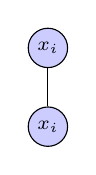
\begin{tikzpicture}[scale=1, main node/.style={circle, draw, fill=blue!20, inner sep=1pt, font=\scriptsize, minimum size=5mm, text=black}]
            % les sommets x_i
            \node[main node] (xi) at (-1,0) {\(x_i\)};
            \node[main node] (bxi) at (-1,-1) {\(\ol{x_i}\)};
            % on connecte les x_i aux bx_i
            \draw (xi) to (bxi);
        \end{tikzpicture}
    }
}